\documentclass{ximera}
%\usepackage{todonotes}

\usepackage{tkz-euclide}
\usetikzlibrary{backgrounds} %% for boxes around graphs
\usetikzlibrary{shapes,positioning}  %% Clouds and stars
\usetkzobj{all}
\usepackage[makeroom]{cancel} %% for strike outs
%\usepackage{mathtools} %% for pretty underbrace % Breaks Ximera
\usepackage{multicol}


\newcommand{\RR}{\mathbb R}
\renewcommand{\d}{\,d}
\newcommand{\dd}[2][]{\frac{d #1}{d #2}}
\renewcommand{\l}{\ell}
\newcommand{\ddx}{\frac{d}{dx}}
\newcommand{\zeroOverZero}{$\boldsymbol{\tfrac{0}{0}}$}
\newcommand{\numOverZero}{$\boldsymbol{\tfrac{\#}{0}}$}
\newcommand{\dfn}{\textbf}
\newcommand{\eval}[1]{\bigg[ #1 \bigg]}
\renewcommand{\epsilon}{\varepsilon}
\renewcommand{\iff}{\Leftrightarrow}

\DeclareMathOperator{\arccot}{arccot}
\DeclareMathOperator{\arcsec}{arcsec}
\DeclareMathOperator{\arccsc}{arccsc}


\colorlet{textColor}{black} 
\colorlet{background}{white}
\colorlet{penColor}{blue!50!black} % Color of a curve in a plot
\colorlet{penColor2}{red!50!black}% Color of a curve in a plot
\colorlet{penColor3}{red!50!blue} % Color of a curve in a plot
\colorlet{penColor4}{green!50!black} % Color of a curve in a plot
\colorlet{penColor5}{orange!80!black} % Color of a curve in a plot
                                      \colorlet{fill1}{blue!50!black!20} % Color of fill in a plot
\colorlet{fill2}{blue!10} % Color of fill in a plot
\colorlet{fillp}{fill1} % Color of positive area
\colorlet{filln}{red!50!black!20} % Color of negative area
\colorlet{gridColor}{gray!50} % Color of grid in a plot

\pgfmathdeclarefunction{gauss}{2}{% gives gaussian
  \pgfmathparse{1/(#2*sqrt(2*pi))*exp(-((x-#1)^2)/(2*#2^2))}%
}



\newcommand{\fullwidth}{}
\newcommand{\normalwidth}{}



%% makes a snazzy t-chart for evaluating functions
\newenvironment{tchart}{\rowcolors{2}{}{background!90!textColor}\array}{\endarray}

%%This is to help with formatting on future title pages.
\newenvironment{sectionOutcomes}{}{} 

\author{Emma Smith Zbarsky}
\license{Creative Commons Attribution 3.0 Unported}
\acknowledgement{https://quadbase.org/questions/q14531v1}
\begin{document}

\begin{exercise}

Find and identify the extrema of $f(x) = \ln(x)-x.$


\begin{hint}
This is an extreme value problem. Because $f$ is continuous on its
domain, $x>0$, we can solve this by only checking the critical points of
$f$ using the second derivative test.
\end{hint}


\begin{hint}
\begin{align*}
f' &= \frac{1}{x}-1 \\
0 &= \frac{1}{x^*}-1 \\
& \Rightarrow x^* = 1 \\
&\\
f'' &= -\frac{1}{x^2} \\
f''(1) &= -\frac{1}{1^2} = -1 <0 \Rightarrow \mbox{ maximum}
\end{align*} There is one extreme value for $f(x) = \ln(x)-x$ -- a
(global) maximum at $x=1$. 

\begin{image}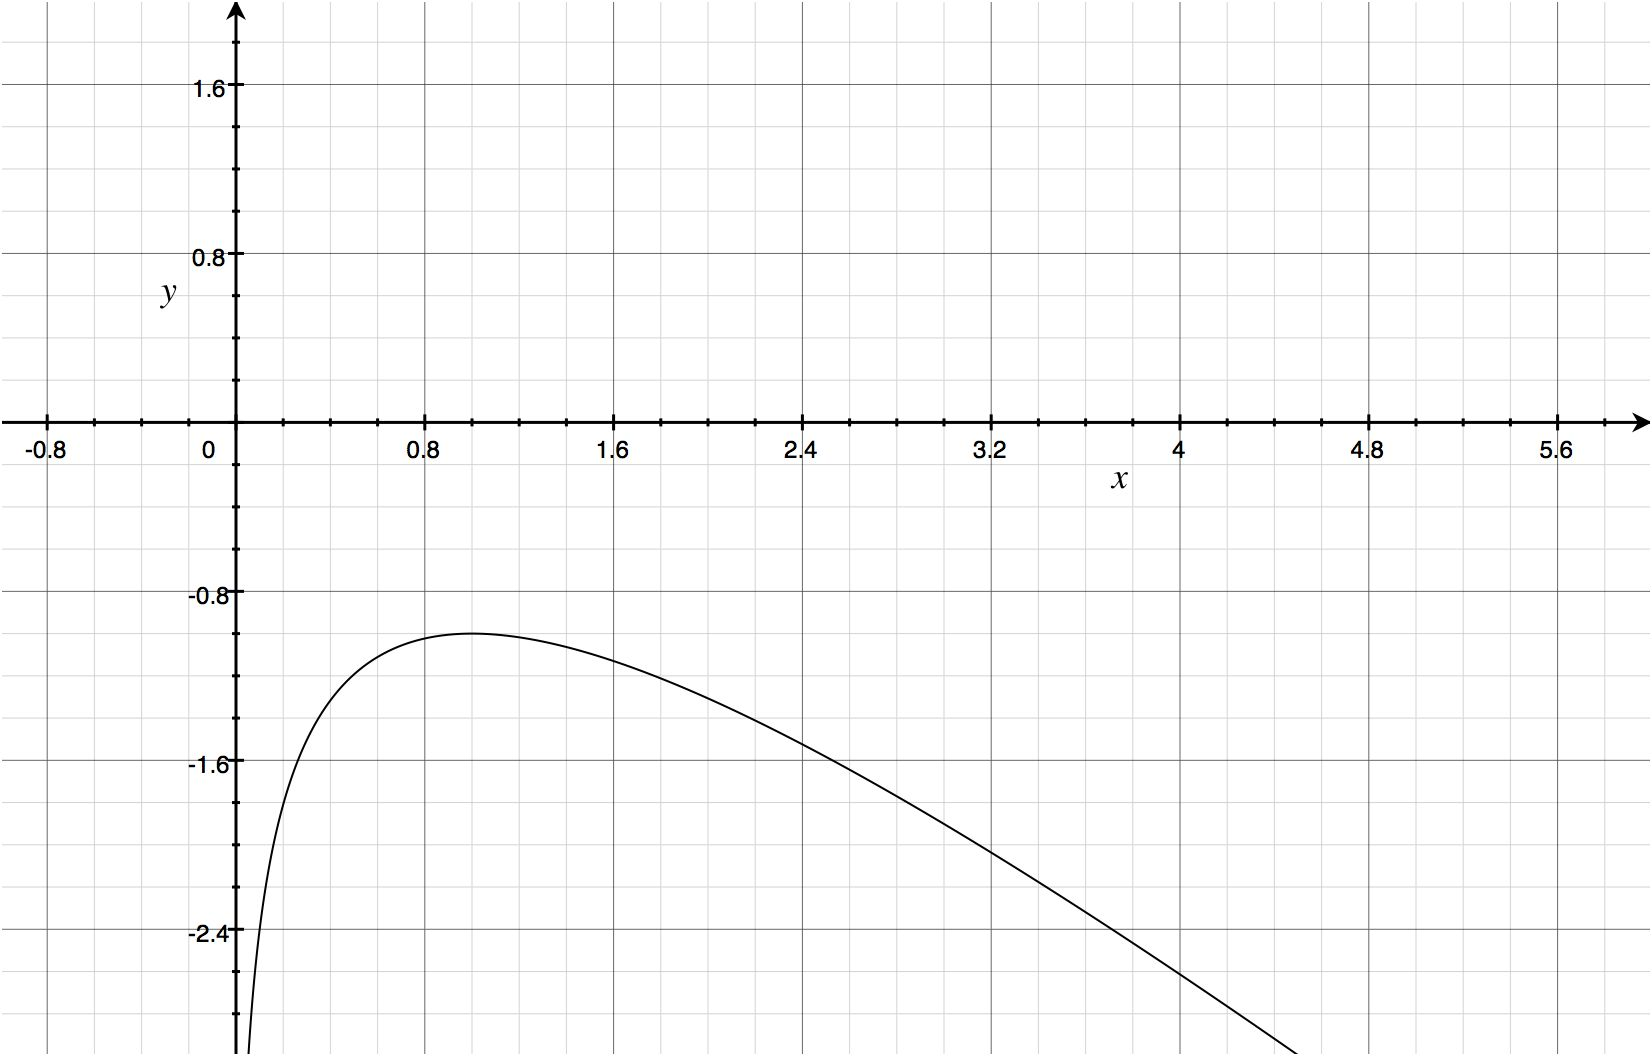
\includegraphics{extremalnx-x.jpg}\end{image}
\end{hint}


\begin{multipleChoice}
\choice[correct]{There is one extremum: a maximum at $x=1$.}
\choice{There are three extrema: a minimum at $x=0$, a maximum at $x=1$ and a
minimum at $x=\infty$.}
\choice{There are no extrema on $f$.}
\choice{There are two extrema: a minimum at $x=0$ and a maximum at $x=1$.}
\choice{There is one extremum: a minimum at $x=1$.}
\end{multipleChoice}

\end{exercise}
\end{document}
